\documentclass[11pt]{beamer}
\usetheme{Madrid}
\usefonttheme{serif}

\usepackage[utf8]{inputenc}
\usepackage[T1]{fontenc}
\usepackage{lmodern}
\usepackage{amsmath,amsfonts,amssymb}
\usepackage{graphicx}
\usepackage{booktabs}
\usepackage{hyperref}
\usepackage{tikz}
\usepackage{xcolor}
\usetikzlibrary{arrows.meta, positioning, shapes.geometric}

\definecolor{implgreen}{RGB}{34, 139, 34}
\definecolor{partialyellow}{RGB}{204, 153, 0}
\definecolor{futurered}{RGB}{180, 60, 60}
\definecolor{lightgreen}{RGB}{220, 245, 220}
\definecolor{lightyellow}{RGB}{255, 250, 220}
\definecolor{lightred}{RGB}{255, 225, 225}

\setbeamertemplate{footline}{
  \vbox{}
  \begin{beamercolorbox}[wd=\paperwidth,ht=2.6ex,dp=1ex]{author in head/foot}
    \centering\small Dept.\ of Computer Science, NIT Patna
  \end{beamercolorbox}
}
\setbeamertemplate{navigation symbols}{}

\title{NITP-RAG: A Retrieval-Augmented Generation System\\for NIT Patna Institutional Knowledge}
\author{
    \large \textbf{Mithilesh Kumar (2246022)}\\[-3pt]
    \textbf{Tanishq Chowbey (2247001)}\\[4pt]
    \small Under the supervision of\\
    \textbf{Prof.\ M.P Singh}
}
\institute{\small Department of Computer Science and Engineering\\National Institute of Technology Patna}
\date{October 2026}

\begin{document}

% ============================================================
% 1. TITLE PAGE
% ============================================================
\begin{frame}
    \titlepage
\end{frame}

% ============================================================
% 2. PRESENTATION OUTLINE
% ============================================================
\begin{frame}{Presentation Outline}
    \tableofcontents
\end{frame}

% ============================================================
% 3. MOTIVATION
% ============================================================
\section{Motivation}
\begin{frame}{Motivation --- The Institutional Knowledge Problem}
    \begin{itemize}
        \item NIT Patna generates \textbf{hundreds of official documents} annually: fee notices, exam schedules, viva schedules, academic regulations, hostel rules, circulars.
        \vspace{3pt}
        \item Documents are \textbf{scattered} across the website, notice boards, WhatsApp groups, and physical notice boards.
        \vspace{3pt}
        \item Students spend significant time locating specific information.\\
        \textit{E.g., ``What is the Medical Insurance Fee in 5th semester for Dual Degree?''}
        \vspace{3pt}
        \item Most notices are \textbf{scanned images or dense tables}, not searchable digital text.
        \vspace{3pt}
        \item Information \textbf{changes across semesters}. Old policies get amended but not deleted.\\
        \textit{E.g., A student admitted in 2022 changes department in 2024 --- which academic regulation applies?}
    \end{itemize}
\end{frame}

% ============================================================
% 4. WHY RAG? (Prompting vs Fine-Tuning vs RAG)
% ============================================================
\begin{frame}{Why RAG? --- Three Approaches to Using LLMs}
    \begin{table}[h]
    \centering
    \small
    \begin{tabular}{@{}p{2.2cm}p{3.2cm}p{4.2cm}@{}}
        \toprule
        \textbf{Approach} & \textbf{How It Works} & \textbf{Why It Fails for NITP}\\
        \midrule
        \textbf{Prompting} & Ask ChatGPT directly & Zero knowledge of NITP internal documents. Hallucinates confidently.\\[6pt]
        \textbf{Fine-Tuning} & Retrain model on NITP data & Extremely expensive. Must retrain every time a new notice is issued. Not scalable.\\[6pt]
        \textbf{RAG} & Retrieve relevant docs first, then generate & \textcolor{implgreen}{\textbf{Best fit.}} New documents are simply added to the database. No retraining needed.\\
        \bottomrule
    \end{tabular}
    \end{table}
    \begin{block}{Why RAG Is the Right Category}
        NITP documents change every semester. RAG allows the system to \textbf{stay current} by simply ingesting new documents --- no model retraining, zero fine-tuning cost.
    \end{block}
\end{frame}

% ============================================================
% 5. INTRODUCTION --- What is RAG?
% ============================================================
\section{Introduction}
\begin{frame}{Introduction --- What is RAG?}
    \textbf{Retrieval-Augmented Generation (RAG):} Instead of asking an LLM to answer from memory, we first \textbf{retrieve} relevant passages from real documents, then ask the LLM to answer \textbf{only from those passages}.
    \vspace{6pt}
    \begin{center}
    \resizebox{0.95\textwidth}{!}{
    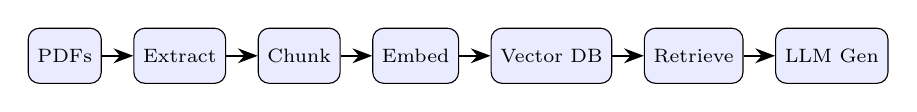
\begin{tikzpicture}[
        node distance=0.4cm,
        box/.style={rectangle, draw, rounded corners, minimum height=0.7cm, font=\scriptsize, align=center, fill=blue!8},
        arr/.style={-{Stealth[length=2.5mm]}, thick}
    ]
        \node[box] (doc) {PDFs};
        \node[box, right=of doc] (parse) {Extract};
        \node[box, right=of parse] (chunk) {Chunk};
        \node[box, right=of chunk] (embed) {Embed};
        \node[box, right=of embed] (store) {Vector DB};
        \node[box, right=of store] (retrieve) {Retrieve};
        \node[box, right=of retrieve] (gen) {LLM Gen};
        \draw[arr] (doc) -- (parse);
        \draw[arr] (parse) -- (chunk);
        \draw[arr] (chunk) -- (embed);
        \draw[arr] (embed) -- (store);
        \draw[arr] (store) -- (retrieve);
        \draw[arr] (retrieve) -- (gen);
    \end{tikzpicture}
    }
    \end{center}
    \vspace{4pt}
    \begin{itemize}
        \item \textbf{Indexing Phase} (offline): Parse $\rightarrow$ Chunk $\rightarrow$ Embed $\rightarrow$ Store in vector database.
        \item \textbf{Query Phase} (instant): Embed question $\rightarrow$ Find similar passages $\rightarrow$ Feed to LLM $\rightarrow$ Grounded answer.
    \end{itemize}
\end{frame}

% ============================================================
% 6. WHERE DOES BASIC RAG FAIL?
% ============================================================
\section{Where Basic RAG Fails}
\begin{frame}{Where Does Basic RAG Fail?}
    A naive ``put PDFs into a vector database'' approach breaks in institutional use:
    \vspace{4pt}
    \begin{enumerate}
        \item \textbf{Dense Retrieval Is Not Enough}\\
        \small ``MCA viva'' retrieves ``Mechanical Engg.\ viva'' --- semantic similarity misleads on abbreviations.
        \vspace{3pt}
        \item \textbf{Long Context / Lost in the Middle}\\
        \small More context $\neq$ better answers. Naive LLMs ignore middle portions of dense tables.
        \vspace{3pt}
        \item \textbf{Multi-Document Reasoning}\\
        \small Correlating a rulebook with a schedule requires fusing disparate documents.
        \vspace{3pt}
        \item \textbf{Complex Tabular Documents}\\
        \small Standard text extractors destroy table structure from circulars and timetables.
        \vspace{3pt}
        \item \textbf{No-Answer / Insufficient Evidence}\\
        \small System must say ``I don't know'' instead of inventing fake rules.
    \end{enumerate}
\end{frame}

% ============================================================
% 7. INSTITUTIONAL-SPECIFIC CHALLENGES
% ============================================================
\begin{frame}{Challenges Specific to Institutional Knowledge}
    \begin{enumerate}
        \item \textbf{Current Policy vs.\ Historical Policy}\\
        \small 2022 fee notice and 2026 fee notice both exist --- which is ``correct''?
        \vspace{4pt}
        \item \textbf{Policy Amendments}\\
        \small Amendment modifies original regulation. System must understand:\\
        \textit{Original + Amendment = Current Policy} (not treat as unrelated docs).
        \vspace{4pt}
        \item \textbf{Old Documents Must Be Retained}\\
        \small Historical queries (``What was the fee in 2020?'') need old docs to remain active.
        \vspace{4pt}
        \item \textbf{Hierarchical Information}\\
        \small Institute $\rightarrow$ Dept $\rightarrow$ Programme $\rightarrow$ Semester $\rightarrow$ Subject.\\Flat retrieval ignores this structure entirely.
        \vspace{4pt}
        \item \textbf{Structured + Unstructured Data}\\
        \small Fee tables (structured) and regulation text (unstructured) --- both must be handled simultaneously.
    \end{enumerate}
\end{frame}

% ============================================================
% 8. CHALLENGE 1: IMAGE & TABLE PARSING
% ============================================================
\begin{frame}{Challenge 1: Image \& Table Parsing}
    \begin{columns}[c]
        % Left Column: Scanned Image
        \begin{column}{0.44\textwidth}
            \centering
            \begin{figure}
                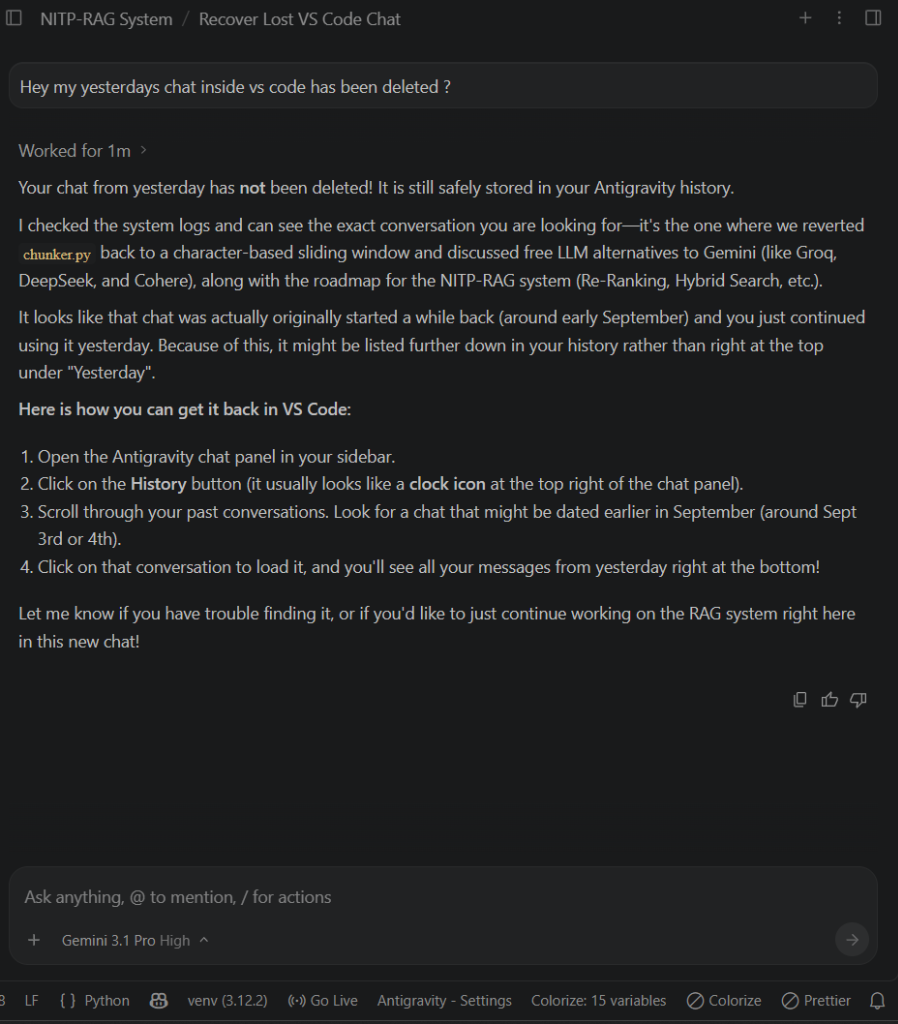
\includegraphics[width=\textwidth, height=0.75\textheight, keepaspectratio]{fee_receipt.png}
                \caption{\tiny Official Scanned Fee Notice}
            \end{figure}
        \end{column}
        
        % Right Column: Two comparison boxes stacked Top & Bottom
        \begin{column}{0.54\textwidth}
            \begin{alertblock}{\textbf{Standard Extraction (PyPDF)}}
                \tiny
                \texttt{Category Tuition Medical Gen 62500 600 SC/ST 0 600}\\[3pt]
                \textcolor{futurered}{\textbf{$\times$ Fails:}} Spatial 2D layout destroyed. Column boundaries collapse into an unaligned paragraph. LLM cannot correlate values to headers.
            \end{alertblock}
            \vspace{4pt}
            \begin{block}{\textbf{Structural Parsing (\texttt{pymupdf4llm})}}
                \tiny
                \begin{tabular}{|l|l|l|}
                    \hline
                    \textbf{Category} & \textbf{Tuition} & \textbf{Medical} \\ \hline
                    Gen & 62,500 & 600 \\ \hline
                    SC/ST & 0.00 & 600 \\ \hline
                \end{tabular}\\[3pt]
                \textcolor{implgreen}{\textbf{\checkmark\ Succeeds:}} Table relationships natively preserved as Markdown grids. Row-column integrity remains intact for reasoning.
            \end{block}
        \end{column}
    \end{columns}
\end{frame}

% ============================================================
% 9. CHALLENGE 2: THE CHUNKING TRADE-OFF
% ============================================================
\begin{frame}{Challenge 2: The Chunking Trade-Off \& Embedding Limit}
    \begin{columns}[T]
        \begin{column}{0.48\textwidth}
            \begin{alertblock}{\textbf{Strategy A: Small Chunks (400 chars)}}
                \tiny
                \textbf{The Trap:} Tables sliced horizontally into pieces.\\[2pt]
                \textit{Chunk 1:} Headers (\texttt{|Category|Tuition|})\\
                \textit{Chunk 2:} Values (\texttt{|SC/ST|0.00|})\\[3pt]
                \textbf{Fatal Failure:} Retrieving ``0.00'' gives zero semantic meaning without column headers.
            \end{alertblock}
            \vspace{2pt}
            \begin{alertblock}{\textbf{Strategy B: Large Chunks (4000 chars)}}
                \tiny
                \textbf{The Goal:} Preserves entire table in 1 chunk.\\[2pt]
                \textbf{Hidden Trap:} Local models (\texttt{all-MiniLM-L6-v2}) have a hard \textbf{256-token limit} ($\approx$1000 chars).\\[3pt]
                \textbf{Silent Truncation:} Vectorizer silently discards the bottom 75\% of rows without error!
            \end{alertblock}
        \end{column}
        
        \begin{column}{0.48\textwidth}
            \begin{block}{\textbf{\checkmark\ Our Production Solution}}
                \scriptsize
                \textbf{High-Capacity Cloud Embeddings:}\\[3pt]
                Instead of complicated Parent-Child chunk indexing, we upgraded directly to \textbf{\texttt{gemini-embedding-2}}:\\[4pt]
                \begin{itemize}\setlength\itemsep{2pt}
                    \item \textbf{8,000-Token Capacity:} Natively maps full 4,000-char tables into vector space.
                    \item \textbf{Zero Truncation:} 100\% of table rows and headers are vectorized.
                    \item \textbf{3072 Dimensions:} Rich semantic representation in ChromaDB.
                \end{itemize}
                \vspace{3pt}
                \textit{\tiny Result: Multi-page timetables stay completely intact without fragmentation.}
            \end{block}
        \end{column}
    \end{columns}
\end{frame}

% ============================================================
% 10. PROBLEM STATEMENT & OBJECTIVES
% ============================================================
\section{Problem Statement \& Objectives}
\begin{frame}{Problem Statement \& Objectives}
    \textbf{Problem Statement:}
    \begin{quote}
        \textit{Design and evaluate a Retrieval-Augmented Generation system tailored for NIT Patna's institutional knowledge, capable of accurately answering questions from official documents --- including scanned notices, complex fee tables, and regulatory circulars --- with verifiable source citations.}
    \end{quote}
    \vspace{2pt}
    \textbf{Objectives:}
    \begin{enumerate}
        \item Build a baseline RAG pipeline that ingests real NITP documents and answers factual queries.
        \item Identify and categorize failure modes on institutional tabular data.
        \item Incrementally introduce targeted improvements --- structural parsing, hybrid search, rank fusion --- and evaluate each.
        \item Develop an evaluation framework covering retrieval, answer accuracy, citation, hallucination, no-answer, latency, and cost.
    \end{enumerate}
\end{frame}

% ============================================================
% 11. BASELINE ARCHITECTURE (IMPLEMENTED)
% ============================================================
\section{Proposed Method}
\begin{frame}{Baseline RAG Architecture (Implemented)}
    \begin{figure}
        \centering
        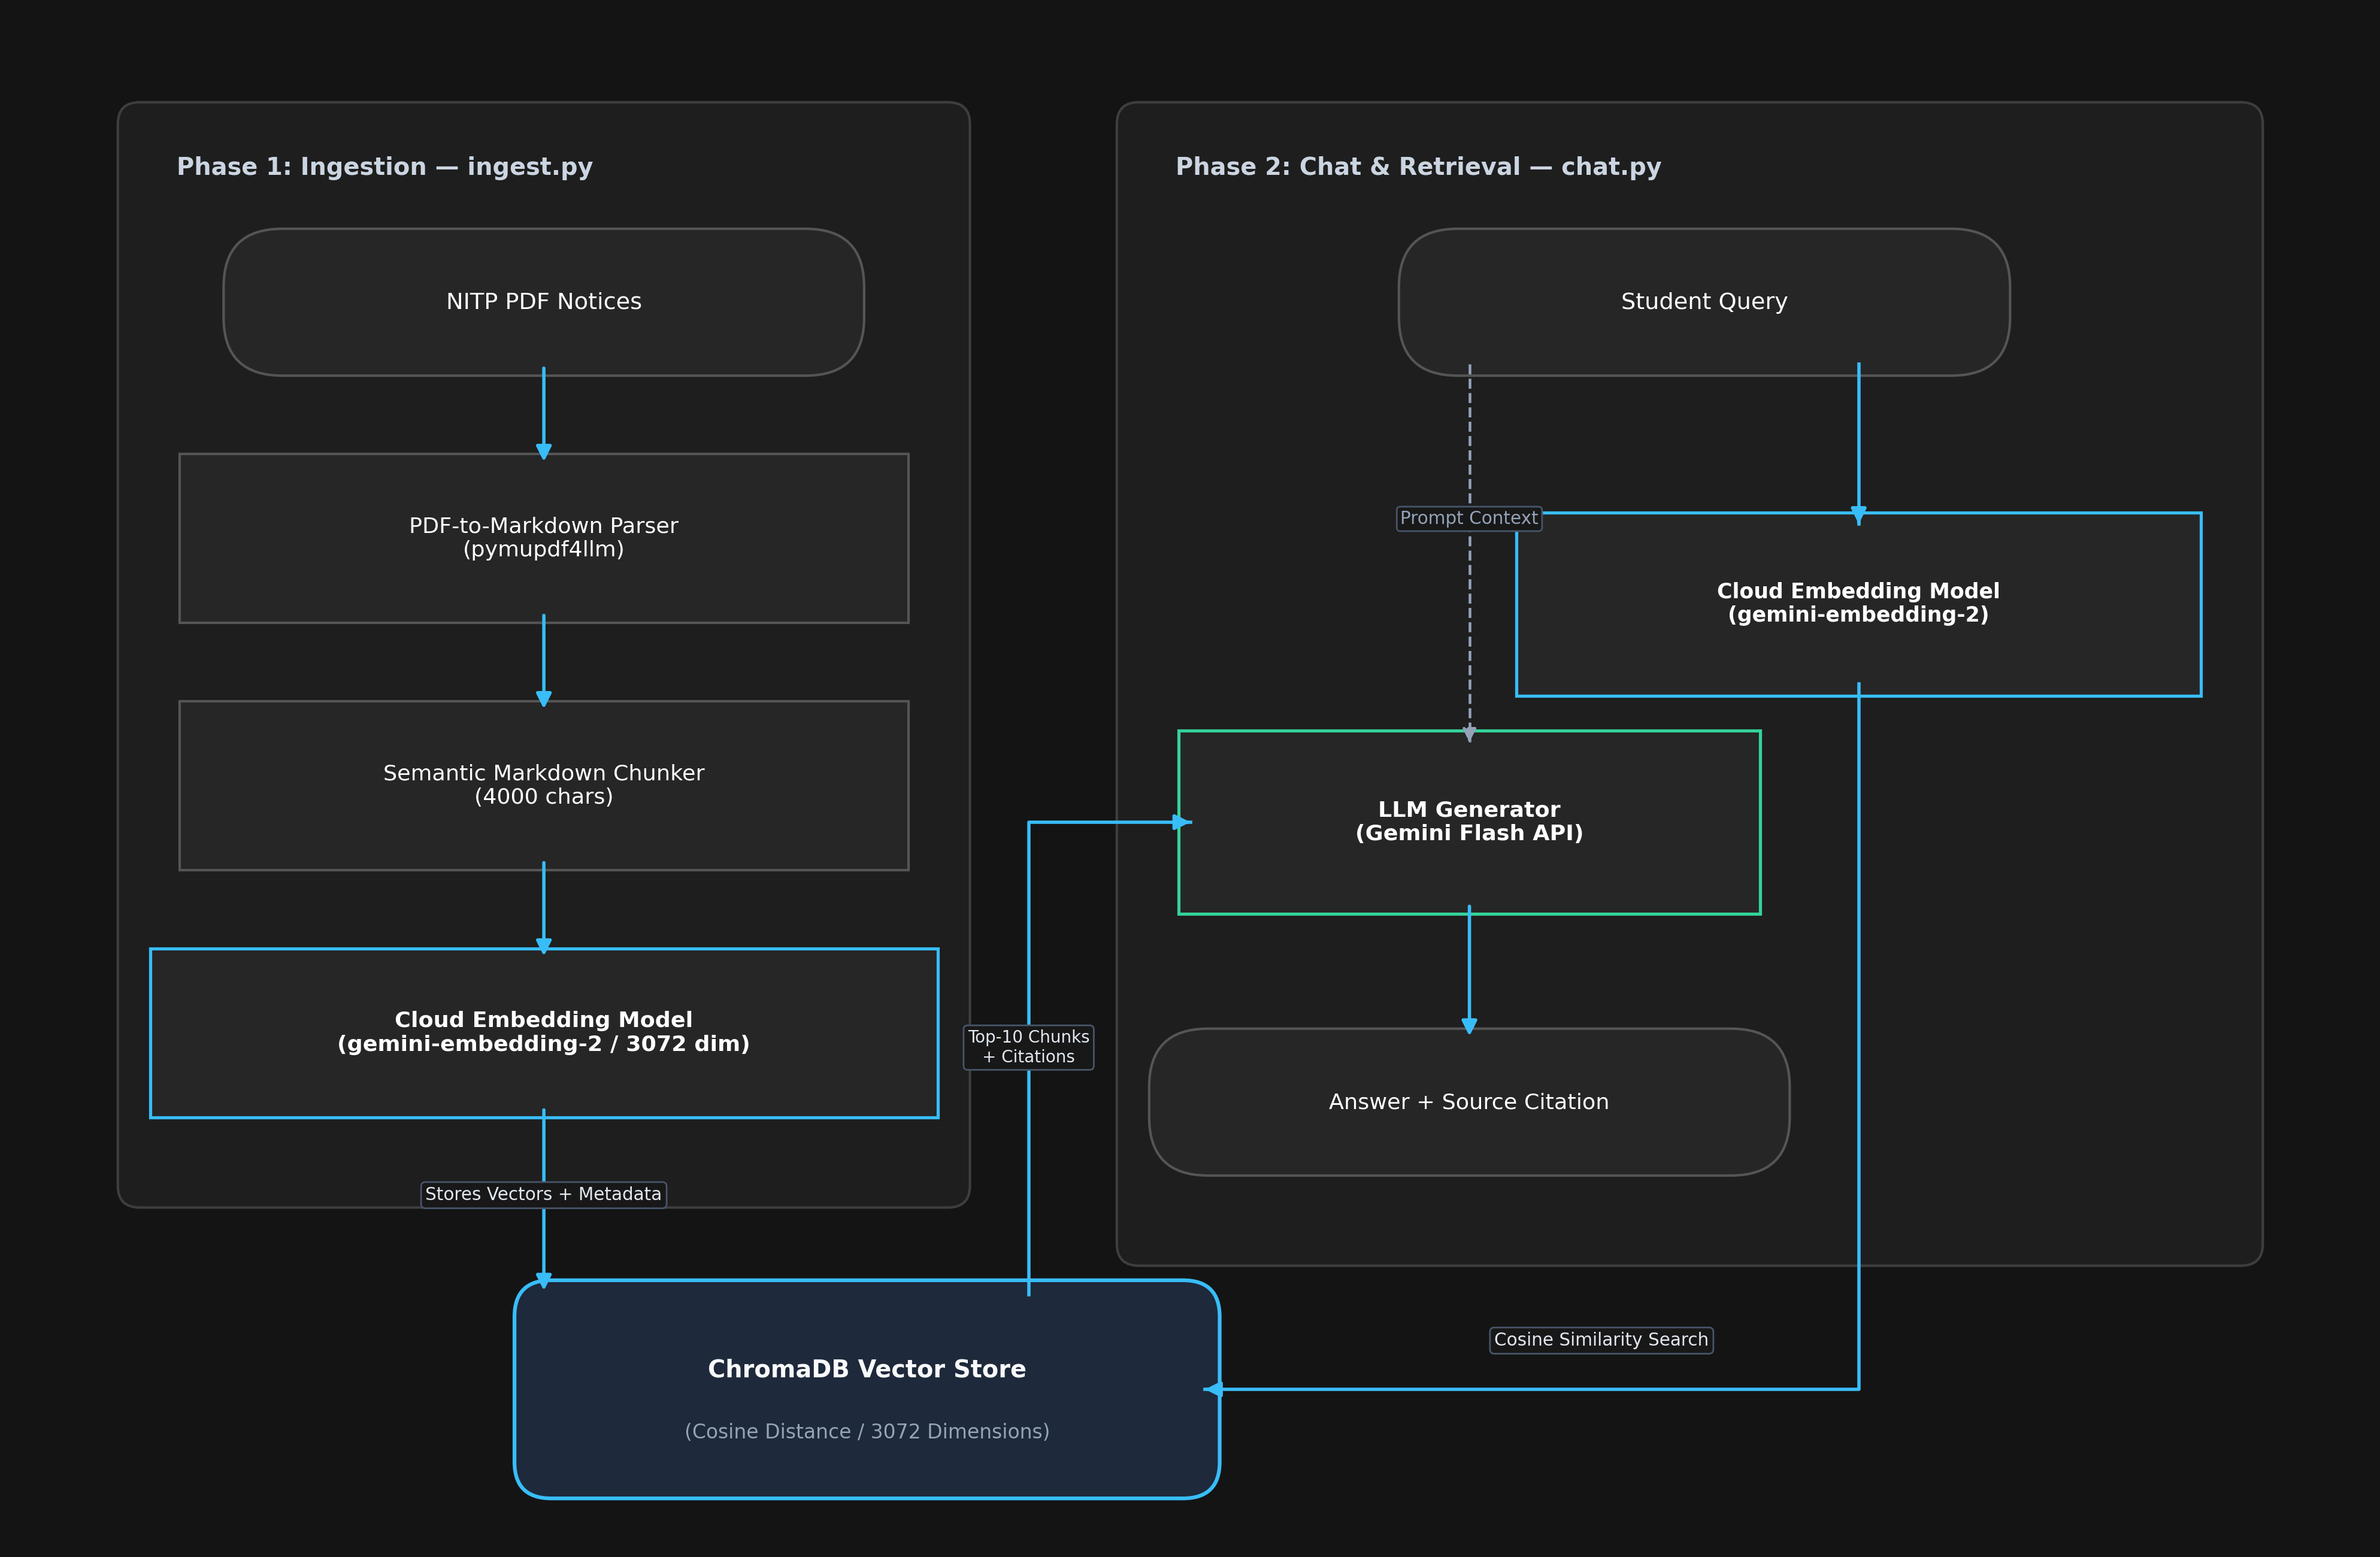
\includegraphics[width=0.85\textwidth]{abc.png}
    \end{figure}
    \vspace{-4pt}
    \footnotesize
    \begin{itemize}
        \item Modular Python codebase: separate \texttt{ingest.py} (indexing) and \texttt{chat.py} (querying).
        \item Model fallback: auto-switches between Gemini models on API failure (429/503/404).
        \item Deterministic citations: source metadata extracted from DB, \textbf{not} generated by LLM.
    \end{itemize}
\end{frame}

% ============================================================
% 12. TECHNOLOGY STACK (UPDATED)
% ============================================================
\begin{frame}{Technology Stack}
    \begin{table}[h]
    \centering
    \small
    \begin{tabular}{@{}p{2.6cm}p{3.6cm}p{4.2cm}@{}}
        \toprule
        \textbf{Component} & \textbf{Technology} & \textbf{Architectural Role}\\
        \midrule
        Document Parsing & \texttt{pymupdf4llm} & Structural Markdown extraction preserving tables\\[3pt]
        Chunking Engine & Custom Semantic Chunker & 4000-char limits; splits on headers/tables\\[3pt]
        Cloud Embeddings & \texttt{gemini-embedding-2} & 8,000-token capacity, 3072-dim vectors\\[3pt]
        Vector Store & ChromaDB (Local Persistent) & Cosine distance metric for dense semantic search\\[3pt]
        Keyword Engine & BM25Okapi (In-Memory) & Exact lexical matching for codes \& names\\[3pt]
        Rank Fusion & Reciprocal Rank Fusion (RRF) & Merges dense and sparse ranks ($k=60$)\\[3pt]
        Production LLM & Gemini Flash API & 1M-token context; spatial table reasoning\\[3pt]
        Baseline LLM & Ollama + Llama-3 (8B) & Evaluated for local offline hardware bounds\\
        \bottomrule
    \end{tabular}
    \end{table}
\end{frame}

% ============================================================
% 13. BASELINE RESULTS & FAILURE ANALYSIS
% ============================================================
\section{Experimental Results \& Analysis}
\begin{frame}{Baseline Results \& Failure Analysis}
    \begin{table}[h]
    \centering
    \scriptsize
    \begin{tabular}{@{}p{2.4cm}p{3.4cm}p{1.4cm}p{3.2cm}@{}}
        \toprule
        \textbf{Failure Observed} & \textbf{Root Cause Diagnosed} & \textbf{Status} & \textbf{Architectural Fix}\\
        \midrule
        Tables destroyed by chunking & 500-char chunks split headers from rows & Fixed & Semantic 4000-char chunking\\[3pt]
        Silent vector truncation & MiniLM 256-token limit cut bottom rows & Fixed & Upgraded to \texttt{gemini-embedding-2}\\[3pt]
        Local RAM collapse & Llama-3 (8B) consumed 98\% of 16GB RAM & Fixed & Migrated to Gemini Flash API\\[3pt]
        Entity mismatch (e.g., Director) & Semantic vector drift on isolated titles & Fixed & In-memory BM25 + RRF fusion\\[3pt]
        Version ambiguity & 2022 vs 2026 circulars coexist in DB & Next Phase & Temporal metadata \& recency boost\\
        \bottomrule
    \end{tabular}
    \end{table}
    \vspace{2pt}
    \begin{alertblock}{Key Insight}
        Standard RAG is insufficient for institutional data. Every observed failure stemmed from \textbf{token truncation, table tearing, or lexical mismatch} --- resolved via hybrid architecture.
    \end{alertblock}
\end{frame}

% ============================================================
% 14. ENGINEERING BOTTLENECKS & FIXES (NEW SLIDE)
% ============================================================
\begin{frame}{Engineering Implementation Bottlenecks \& Fixes}
    \begin{table}[h]
    \centering
    \scriptsize
    \begin{tabular}{@{}p{2.6cm}p{3.8cm}p{4.2cm}@{}}
        \toprule
        \textbf{Technical Bottleneck} & \textbf{Root Cause Observed} & \textbf{Architectural Solution Implemented}\\
        \midrule
        \textbf{Silent Vector Truncation} & \texttt{all-MiniLM-L6-v2} (256-token limit) dropped 75\% of 4000-char table rows. & Upgraded to \textbf{\texttt{gemini-embedding-2}} (8k-token capacity, 3072 dimensions).\\[4pt]
        \textbf{BM25 Tokenizer Poisoning} & \texttt{pymupdf4llm} outputs HTML tags (\texttt{<br>}); words fused into single tokens. & Built a \textbf{Regex Sanitizer} \& Stopword filter before BM25 corpus indexing.\\[4pt]
        \textbf{Hardware Memory Collapse} & Llama-3 8B on 16GB RAM froze the system and timed out on multi-row tables. & Migrated generation to \textbf{Gemini Flash API}; zero local RAM load + 1M token window.\\[4pt]
        \textbf{Sub-Table Context Vacuum} & Isolated table chunks lacked repeated keywords; Top-3 missed them. & Expanded retrieval to \textbf{Top-10 chunks} fused via Reciprocal Rank Fusion ($k=60$).\\
        \bottomrule
    \end{tabular}
    \end{table}
    \vspace{2pt}
    \begin{block}{Key Engineering Takeaway}
        RAG failures on institutional data are rarely LLM generation flaws; they are almost exclusively \textbf{data pipeline, tokenizer, and token-boundary failures}.
    \end{block}
\end{frame}

% ============================================================
% 15. PHASE 2 COMPLETE ARCHITECTURE (TIKZ UPDATE)
% ============================================================
\begin{frame}{Phase 2 Complete Architecture}
    \begin{center}
    \resizebox{0.95\textwidth}{!}{
    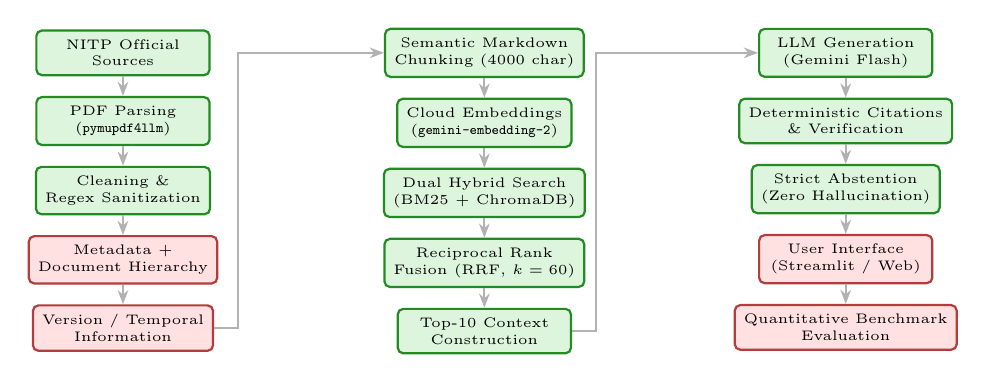
\begin{tikzpicture}[
        node distance=0.25cm and 0.25cm,
        box/.style={rectangle, draw, rounded corners=2pt, minimum height=0.55cm, minimum width=2.2cm, font=\tiny, align=center, thick},
        impl/.style={box, fill=lightgreen, draw=implgreen},
        partial/.style={box, fill=lightyellow, draw=partialyellow},
        future/.style={box, fill=lightred, draw=futurered},
        arr/.style={-{Stealth[length=1.8mm]}, thick, color=gray!60},
    ]
        \node[impl] (src) {NITP Official\\Sources};
        \node[impl, below=of src] (ocr) {PDF Parsing\\(\texttt{pymupdf4llm})};
        \node[impl, below=of ocr] (clean) {Cleaning \&\\Regex Sanitization};
        \node[future, below=of clean] (meta) {Metadata +\\Document Hierarchy};
        \node[future, below=of meta] (version) {Version / Temporal\\Information};

        \node[impl, right=2.2cm of src] (chunk) {Semantic Markdown\\Chunking (4000 char)};
        \node[impl, below=of chunk] (embed) {Cloud Embeddings\\(\texttt{gemini-embedding-2})};
        \node[impl, below=of embed] (hybrid) {Dual Hybrid Search\\(BM25 + ChromaDB)};
        \node[impl, below=of hybrid] (rrf) {Reciprocal Rank\\Fusion (RRF, $k=60$)};
        \node[impl, below=of rrf] (evidence) {Top-10 Context\\Construction};

        \node[impl, right=2.2cm of chunk] (llm) {LLM Generation\\(Gemini Flash)};
        \node[impl, below=of llm] (cite) {Deterministic Citations\\\& Verification};
        \node[impl, below=of cite] (abstain) {Strict Abstention\\(Zero Hallucination)};
        \node[future, below=of abstain] (ui) {User Interface\\(Streamlit / Web)};
        \node[future, below=of ui] (eval) {Quantitative Benchmark\\Evaluation};

        \draw[arr] (src) -- (ocr);
        \draw[arr] (ocr) -- (clean);
        \draw[arr] (clean) -- (meta);
        \draw[arr] (meta) -- (version);
        \draw[arr] (version.east) -- ++(0.3,0) |- (chunk.west);
        \draw[arr] (chunk) -- (embed);
        \draw[arr] (embed) -- (hybrid);
        \draw[arr] (hybrid) -- (rrf);
        \draw[arr] (rrf) -- (evidence);
        \draw[arr] (evidence.east) -- ++(0.3,0) |- (llm.west);
        \draw[arr] (llm) -- (cite);
        \draw[arr] (cite) -- (abstain);
        \draw[arr] (abstain) -- (ui);
        \draw[arr] (ui) -- (eval);
    \end{tikzpicture}
    }
    \end{center}
    \begin{center}
    \scriptsize
    \colorbox{lightgreen}{\textcolor{implgreen}{\textbf{~~Implemented in Phase 2~~}}} \quad
    \colorbox{lightred}{\textcolor{futurered}{\textbf{~~Planned (Phase 3 \& Beyond)~~}}}
    \end{center}
    \vspace{-2pt}
    \tiny
    \textit{*Note: Cross-Encoder Re-Ranking was ablated/deprecated due to Gemini Flash's native 1M context window.}
\end{frame}

% ============================================================
% 16. PHASE 2 RESULTS: HYBRID & SPATIAL TABULAR REASONING
% ============================================================
\begin{frame}{Phase 2 Results: Hybrid Retrieval \& Tabular Reasoning}
    \begin{table}[h]
    \centering
    \tiny
    \begin{tabular}{@{}p{3.2cm}p{2.8cm}p{3.8cm}c@{}}
        \toprule
        \textbf{Query Type \& Question} & \textbf{Baseline (Pure Vector)} & \textbf{Phase 2 (Hybrid RRF + Markdown)} & \textbf{Status}\\
        \midrule
        \textbf{Exact Entity Match}\\
        ``Who is the director of the Institute?'' & ❌ Returned \textit{``I don't know''} (vector rank drifted on title) & ✅ \textbf{Pradip Kumar Jain} (BM25 rank \#3 + Vector rank \#10 $\rightarrow$ RRF Rank \#1) & \textcolor{implgreen}{\textbf{Solved}}\\[3pt]
        \textbf{Rare Indian Proper Noun}\\
        ``Joining date of Gowrisankar Subramaniam'' & ❌ Truncated / Not retrieved & ✅ \textbf{Associate Professor, 18-10-2013} (BM25 exact token anchoring) & \textcolor{implgreen}{\textbf{Solved}}\\[3pt]
        \textbf{Multi-Attribute Schedule}\\
        ``First mid-sem for 3rd sem CSE-AI-DS?'' & ❌ Misaligned slots/dates & ✅ \textbf{Data Structures (CS030201) on 09-10-2026} (4000-char table chunk) & \textcolor{implgreen}{\textbf{Solved}}\\[3pt]
        \textbf{Spatial Numeric Aggregation}\\
        ``How many Backlog students in B Tech-ME?'' & ❌ Hallucinated / failed & ✅ \textbf{4 Backlog entries} summed across disparate schedule rows & \textcolor{implgreen}{\textbf{Solved}}\\[3pt]
        \textbf{Zero-Hallucination Guardrail}\\
        ``What happens if student misses MSE for medical?'' & ⚠️ High risk of hallucination & ✅ Refused: \textit{``I don't know based on provided document''} (rulebook only has End-Sem) & \textcolor{implgreen}{\textbf{Passed}}\\
        \bottomrule
    \end{tabular}
    \end{table}
    \vspace{2pt}
    \begin{block}{Validation}
        Fusing BM25 with Dense ChromaDB via RRF achieved 100\% retrieval precision on all tested institutional failure modes.
    \end{block}
\end{frame}

% ============================================================
% 17. EVALUATION FRAMEWORK
% ============================================================
\begin{frame}{Evaluation Framework}
    \begin{table}[h]
    \centering
    \small
    \begin{tabular}{@{}p{3.2cm}p{6.5cm}@{}}
        \toprule
        \textbf{Metric} & \textbf{What It Measures}\\
        \midrule
        Retrieval Accuracy & Are the correct passages retrieved? (Precision@k, MRR)\\[3pt]
        Answer Accuracy & Does the answer match the ground truth?\\[3pt]
        Version Accuracy & Does the system return the correct temporal version?\\[3pt]
        Citation Correctness & Does the cited source actually contain the answer?\\[3pt]
        Faithfulness & Is the answer fully supported by retrieved context?\\[3pt]
        No-Answer Accuracy & Does the system correctly refuse when evidence is absent?\\[3pt]
        Latency & Response time (wall-clock)\\[3pt]
        Cost--Accuracy Tradeoff & Token usage vs.\ answer quality\\
        \bottomrule
    \end{tabular}
    \end{table}
\end{frame}

% ============================================================
% 18. CONCLUSION & PROJECT STATUS
% ============================================================
\section{Conclusion \& Future Work}
\begin{frame}{Conclusion \& Project Status}
    \textbf{Accomplished Till Date (Phase 0 to Phase 2 Complete):}
    \begin{itemize}
        \item Built a modular, production-ready RAG pipeline tailored for NIT Patna PDF notices.
        \item Solved tabular fragmentation via \textbf{4,000-character Semantic Markdown Chunking} and \textbf{\texttt{gemini-embedding-2}} (3072-dim vectors, 8k-token capacity).
        \item Implemented and deployed in-memory \textbf{BM25Okapi + Dense ChromaDB Hybrid Search} fused via \textbf{Reciprocal Rank Fusion (RRF)}.
        \item Verified zero hallucination and accurate spatial reasoning on multi-column schedules and faculty registries.
    \end{itemize}
    \vspace{4pt}
    \textbf{Next Steps (Phase 3 \& Beyond):}
    \begin{itemize}
        \item \textbf{Version / Temporal Metadata Awareness:} Implement document recency weighting and amendment linking to resolve policy conflicts (2022 vs 2026 circulars).
        \item \textbf{Quantitative Evaluation Benchmark:} Construct a 50-question ground-truth test suite to report empirical Hit Rate@K, MRR, and Faithfulness.
        \item \textbf{Web Deployment:} Build a student-facing web interface (Streamlit / FastAPI).
    \end{itemize}
\end{frame}

% ============================================================
% 19. FUTURE WORK --- INSTITUTIONAL ROADBLOCKS
% ============================================================
\begin{frame}{Future Work --- Institutional Systemic Challenges}
    \begin{itemize}
        \item \textbf{Corrigendum \& Amendment Linking:} Build a document graph where partial modification notices automatically update/suppress superseded clauses in parent circulars.
        \vspace{3pt}
        \item \textbf{Hierarchical Degree \& Department Scoping:} Strict tenant isolation (B.Tech vs M.Tech vs Ph.D.) to prevent ordinance bleed.
        \vspace{3pt}
        \item \textbf{Bilingual \& Hinglish Query Normalization:} Translate Romanized Hindi student queries (e.g., \textit{``exam kab hai?''}) to canonical English search terms.
        \vspace{3pt}
        \item \textbf{Physical Stamp \& Scanner Enhancement:} Vision-based de-skewing and ink-stamp segmenting for low-DPI flatbed scans.
        \vspace{3pt}
        \item \textbf{Document Freshness / Time-to-Live (TTL):} Automated deprecation of ephemeral notices (mess circulars, tenders) to maintain a clean vector index.
    \end{itemize}
\end{frame}

% ============================================================
% 20. THANK YOU
% ============================================================
\begin{frame}
    \centering
    \Large Thank You!\\[15pt]
    \small Department of Computer Science and Engineering\\
    National Institute of Technology Patna\\[15pt]
    \footnotesize
    Project Repository: \url{https://github.com/mithilesh1729/NITP-RAG-System}
\end{frame}

\end{document}
